\chapter{\label{ch2-mechanics}Camera Design \& Mechanics}

\minitoc

\notes[inline,caption={}]{
	\section{Plan}
	\subsection{Topics}
	\begin{itemize}
		\item Introduce TARGET architecture \& Wilkinson ADC
		\item Different TARGET versions
		\item FEE
		\item MAPMs
		\item SiPMS
		\begin{itemize}
			\item How they work
			\item Comparison investigations
			\item Property trade-offs
		\end{itemize}
		\item CHEC-M
		\item Changes for CHEC-S
		\item Future - MUSIC ASICs
	\end{itemize}
	\subsection{Questions}
	\begin{itemize}
		\item ?
	\end{itemize}
}

\section{Introduction}


\section{CHEC-M}

\subsection{Multi-Anode Photomultiplier Tubes}

\subsection{Front-End Electronics}

\subsubsection{Pre-Amplifiers}

\subsubsection{TARGET}

\begin{figure}
	\centering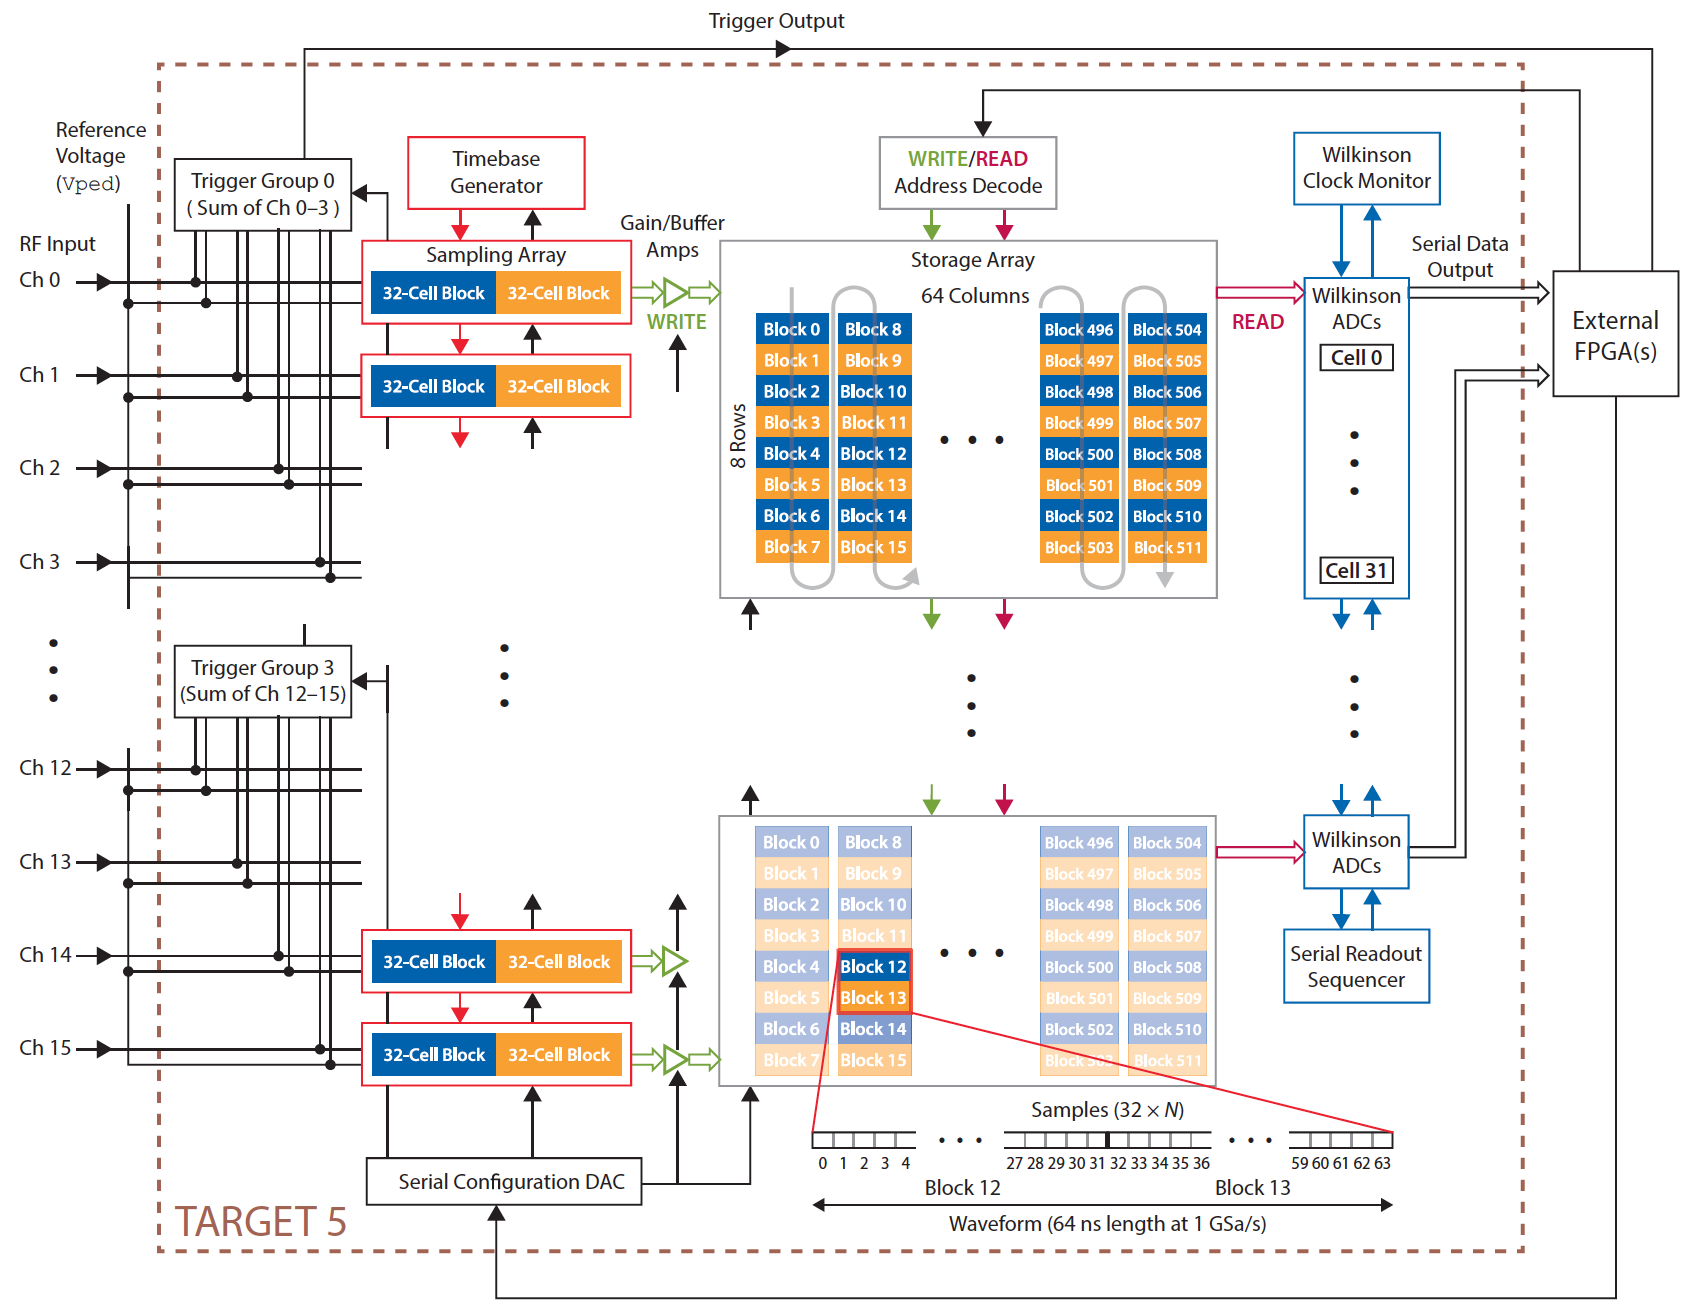
\includegraphics[width=\textwidth]{target5diagram} 
	\caption[Functional block diagram of the TARGET~5 ASIC.]{Functional block diagram of the TARGET~5 ASIC \cite{Albert2017} \change[inline]{Add more details}}
	\label{fig:target5diagram}
\end{figure}

\subsection{Back-End Electronics}

\subsubsection{Backplane}

\subsubsection{DACQ Boards}

\subsection{Peripherals\change{?}}

\subsubsection{LED Flashers}

\subsubsection{Chiller}

\section{CHEC-S}

\subsection{Silicon Photomultipliers}

\subsection{TARGET-C}

\change[inline]{larger dynamic range, reference tf plot????}

\change{name of TARGET-C FPGA?}

\section{Future}

\section{Lab Set-Up}

\section{Readout Characteristics}

\change{define ADC}